\documentclass{beamer}
\mode<presentation>
{
  \usetheme{Madrid}
  \usecolortheme{crane}
  \usefonttheme{structurebold}
  \setbeamertemplate{navigation symbols}{}
  \setbeamertemplate{caption}[numbered]
} 

\usepackage[russian]{babel}
\usepackage[utf8x]{inputenc}

\title[Структура ПО]{Структура программного обеспечения компьютера}
\author{Селянин А.И.}
\institute{585 группа}
\date{30.04.2020}

\begin{document}

\begin{frame}
  \titlepage
\end{frame}

\section{Introduction}

\begin{frame}{Структура ПО}

\begin{block}{Определение}
Совокупность программ, предназначенная для решения задач на ПК, называется программным обеспечением. Состав  программного обеспечения ПК называют программной конфигурацией.
\end{block}

\vskip 0,5cm

\begin{itemize}
  \item Системное ПО
  \item Прикладное ПО
  \item Инструментарий технологий программирования
\end{itemize}

\end{frame}

\subsection{Структура ПО}

\begin{frame}{Структура ПО}

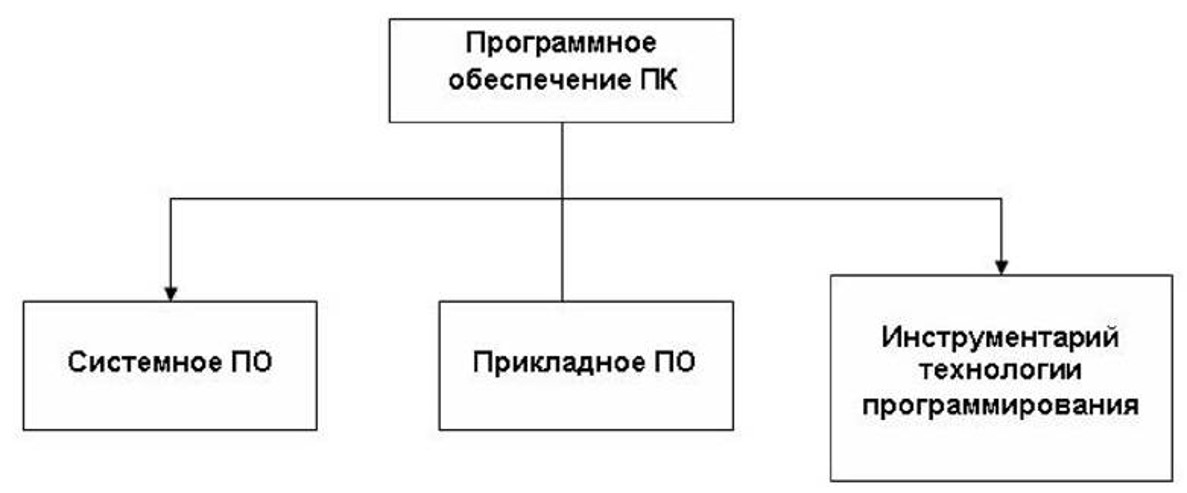
\includegraphics[width=1\linewidth]{22.jpg}

\end{frame}

\begin{frame}

\vskip 0,5cm

К системному ПО относятся:
\begin{enumerate} 
  \item операционные системы 
  \item программы – оболочки
  \item операционные оболочки
  \item драйверы
  \item утилиты
\end{enumerate}

\end{frame}

\begin{frame}

Необходимо отметить, что часть утилит входит в состав операционной системы, а другая часть функционирует автономно. Большая часть общего (системного) ПО входит в состав ОС. Часть общего ПО входит в состав самого компьютера (часть программ ОС и контролирующих тестов записана в ПЗУ или ППЗУ, установленных на системной плате). Часть общего ПО относится к автономными программам и поставляется отдельно.

\end{frame}

\begin{frame}
    
\begin{table}[]
\begin{tabular}{|l|l|l|l|}
\hline
\multicolumn{4}{|l|}{Таблица 1}                    \\ \hline
\multicolumn{2}{|l|}{A2} & \multicolumn{2}{l|}{B2} \\ \hline
\multicolumn{2}{|l|}{A3} & \multicolumn{2}{l|}{B3} \\ \hline
\end{tabular}
\end{table}

\[H=-\sum_{i=1}^{n}p_{i}log_{2}p_{i}\]
    
\end{frame}

\end{document}
